\documentclass[a4paper,12pt]{article}
\usepackage[utf8]{inputenc}
\usepackage[spanish]{babel}
\usepackage{color}
\usepackage{parskip}
\usepackage{graphicx}
\usepackage{multirow}
\usepackage{listings}
\usepackage{vmargin}
\graphicspath{ {imagenes/} }
\definecolor{mygreen}{rgb}{0,0.6,0}
\definecolor{lbcolor}{rgb}{0.9,0.9,0.9}
\usepackage{epstopdf}


\setpapersize{A4}
\setmargins{2.5cm}       % margen izquierdo
{1.5cm}                        % margen superior
{16.5cm}                      % anchura del texto
{23.42cm}                    % altura del texto
{10pt}                           % altura de los encabezados
{1cm}                           % espacio entre el texto y los encabezados
{0pt}                             % altura del pie de página
{2cm}     

\lstset{
%backgroundcolor=\color{lbcolor},
    tabsize=4,    
%   rulecolor=,
    language=[GNU]C++,
        basicstyle=\tiny,
        aboveskip={1.5\baselineskip},
        columns=fixed,
        showstringspaces=false,
        extendedchars=false,
        breaklines=true,
        prebreak = \raisebox{0ex}[0ex][0ex]{\ensuremath{\hookleftarrow}},
        frame=single,
        showtabs=false,
        showspaces=false,
        showstringspaces=false,
        identifierstyle=\ttfamily,
        keywordstyle=\color[rgb]{0,0,1},
        commentstyle=\color[rgb]{0.026,0.112,0.095},
        stringstyle=\color{red},
        numberstyle=\color[rgb]{0.205, 0.142, 0.73},
%        \lstdefinestyle{C++}{language=C++,style=numbers}’.
}

\begin{document}
\begin{titlepage}

\begin{center}
\vspace*{-1in}

\begin{large}
UNIVERSIDAD NACIONAL DE SAN AGUSTÍN\\
\vspace*{0.15in}
ESCUELA PROFESIONAL DE CIENCIA DE LA COMPUTACIÓN\\
\end{large}
\begin{figure}[htb]
\centering

\includegraphics[scale=0.13]{/home/xnpio/Documentos/Caratula/logo.eps}
\end{figure}
\vspace*{0.15in}
\begin{large}
TEMA:\\
\end{large}
\vspace*{0.2in}
\begin{Large}
\textbf{QR ALGORITHM IN C++} \\
\end{Large}
\vspace{8mm}

\begin{large}
Curso:\\
\end{large}
\vspace*{0.2in}
\begin{Large}
\textbf{MATEMÁTICA APLICADA A LA COMPUTACIÓN} \\
\end{Large}

\vspace{8mm}

\begin{large}
\textbf{Presentado por:}\\

\begin{flushleft}

\hspace{7cm} Christofer Chávez Carazas \\

\end{flushleft}
\end{large}
\vspace{4cm}
\rule{80mm}{0.1mm}\\
\vspace*{0.1in}

\begin{large}
Arequipa - Perú \\
2017 \\
\end{large}
\end{center}
\end{titlepage}


\section{Código}
 \begin{lstlisting}
#include <iostream>
#include <tuple>
#include "OperacionesMatriz.h"

using namespace std;

Num MulList(Lista A, Lista B){
	Num res = 0;
	for(int i = 0; i < A.size(); i++){
		res += A[i] * B[i];
	}
	return res;
}

vector<Lista> getColumns(Matriz & A){
	vector<Lista> res;
	for(int i = 0; i < A.size(); i++){
		Lista temp;
		for(int j = 0; j < A.size(); j++){
			temp.push_back(A[j][i]);
		}
		res.push_back(temp);
	}
	return res;
}

Matriz generarMatriz(vector<Lista> E, int tam){
	Matriz Q = zeros(tam);
	for(int i = 0; i < tam; i++){
		for(int j = 0; j < tam; j++){
			Q[j][i] = E[i][j];
		}
	}
	return Q;
}

tuple<Matriz,Matriz> QRdescomposition(Matriz & A){
	vector<Lista> Es;
	Matriz Q = zeros(A.size());
	Matriz R = zeros(A.size());
	vector<Lista> As = getColumns(A);
	for(int i = 0; i < A.size(); i ++){
		Lista u = As[i];
		for(int j = 0; j < i; j++){
			Num temp = MulList(As[i],Es[j]);
			R[j][i] = temp;
			Lista lTemp = Es[j] * temp;
			u = u - lTemp;
		}
		Es.push_back(u * (1.0/norm(u)));
		R[i][i] = MulList(As[i],Es[i]);
	}
	Q = generarMatriz(Es,A.size());
	return make_tuple(Q,R);
}

int main(int argc, char * argv[]){
	if(argc != 2){
		cout<<"Faltan argumentos <Numero de iteraciones"<<endl;
		return 0;
	}
	string temp(argv[1]);
	int n = stoi(temp);
	Matriz A = {{3,8,1},{2,3,8},{0,2,1}};
	cout<<"Matriz Original:"<<endl;
	mostrarMatriz(A);
	for(int i = 0; i < n; i++){
		auto Q_R = QRdescomposition(A);		
		Matriz Q = get<0>(Q_R);
		Matriz R = get<1>(Q_R);
		A = R * Q;
		cout<<"Iteracion "<<i+1<<":"<<endl;
		mostrarMatriz(A);
	}
}
 \end{lstlisting}
 
 \section{Ejemplo}
 
El ejemplo mostrado se realiza con la siguiente matriz:
 
 \[ A = \left[ \begin{array}{ccc}
3 & 8 & 1 \\
2 & 3 & 8 \\
0 & 2 & 1 \end{array} \right]\] 
 
 \textbf{Número de iteraciones:} $5$
 
\section{Resultados}

Se muestra el resultado de cada iteración.

\begin{figure}[h]
 \centering
 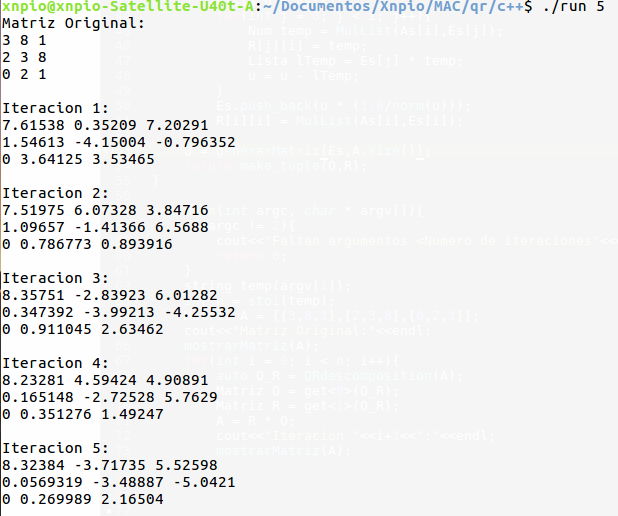
\includegraphics[scale=0.5]{1.png}
\end{figure}


 
\end{document}

